%%%%%%%%%%%%%%%%%%%%%%%%%%%%%%%%%%%%%%%%%
% Journal Article
% LaTeX Template
% Version 1.4 (15/5/16)
%
% This template has been downloaded from:
% http://www.LaTeXTemplates.com
%
% Original author:
% Frits Wenneker (http://www.howtotex.com) with extensive modifications by
% Vel (vel@LaTeXTemplates.com)
%
% License:
% CC BY-NC-SA 3.0 (http://creativecommons.org/licenses/by-nc-sa/3.0/)
%
%%%%%%%%%%%%%%%%%%%%%%%%%%%%%%%%%%%%%%%%%

%----------------------------------------------------------------------------------------
%   PACKAGES AND OTHER DOCUMENT CONFIGURATIONS
%----------------------------------------------------------------------------------------

\documentclass[twoside,twocolumn]{article}

\usepackage{blindtext} % Package to generate dummy text throughout this template

\usepackage[sc]{mathpazo} % Use the Palatino font
\usepackage[T1]{fontenc} % Use 8-bit encoding that has 256 glyphs
\linespread{1.05} % Line spacing - Palatino needs more space between lines
\usepackage{microtype} % Slightly tweak font spacing for aesthetics

\usepackage[english]{babel} % Language hyphenation and typographical rules

\usepackage[hmarginratio=1:1,top=32mm,columnsep=20pt]{geometry} % Document margins
\usepackage[hang, small,labelfont=bf,up,textfont=it,up]{caption} % Custom captions under/above floats in tables or figures
\usepackage{booktabs} % Horizontal rules in tables

\usepackage{lettrine} % The lettrine is the first enlarged letter at the beginning of the text

\usepackage{enumitem} % Customized lists
\setlist[itemize]{noitemsep} % Make itemize lists more compact

\usepackage{abstract} % Allows abstract customization
\renewcommand{\abstractnamefont}{\normalfont\bfseries} % Set the "Abstract" text to bold
\renewcommand{\abstracttextfont}{\normalfont\small\itshape} % Set the abstract itself to small italic text

\usepackage{titlesec} % Allows customization of titles
\renewcommand\thesection{\Roman{section}} % Roman numerals for the sections
\renewcommand\thesubsection{\roman{subsection}} % roman numerals for subsections
\titleformat{\section}[block]{\large\scshape\centering}{\thesection.}{1em}{} % Change the look of the section titles
\titleformat{\subsection}[block]{\large}{\thesubsection.}{1em}{} % Change the look of the section titles

\usepackage{fancyhdr} % Headers and footers
\pagestyle{fancy} % All pages have headers and footers
\fancyhead{} % Blank out the default header
\fancyfoot{} % Blank out the default footer
\fancyhead[C]{Music Generation $\bullet$ November 2018 $\bullet$ Tang, Xu, Xu} % Custom header text
\fancyfoot[RO,LE]{\thepage} % Custom footer text

\usepackage{titling} % Customizing the title section

\usepackage{hyperref} % For hyperlinks in the PDF
\usepackage{url}
\usepackage{graphicx}
\graphicspath{ {./images/}}

%----------------------------------------------------------------------------------------
%   TITLE SECTION
%----------------------------------------------------------------------------------------

\setlength{\droptitle}{-4\baselineskip} % Move the title up

\pretitle{\begin{center}\Huge\bfseries} % Article title formatting
\posttitle{\end{center}} % Article title closing formatting
\title{Music Generation with LSTMs} % Article title
\author{%
\textsc{Joyce Xu} \\[1ex] % Your name
\normalsize Stanford University \\ % Your institution
\normalsize \href{mailto:jexu@stanford.edu}{jexu@stanford.edu} % Your email address
\and % Uncomment if 2 authors are required, duplicate these 4 lines if more
\textsc{Sam Xu} \\[1ex] % Second author's name
\normalsize Stanford University \\ % Second author's institution
\normalsize \href{mailto:samx}{samx@stanford.edu} % Second author's email address
\and % Uncomment if 2 authors are required, duplicate these 4 lines if more
\textsc{Eric Tang} \\[1ex] % Second author's name
\normalsize Stanford University \\ % Second author's institution
\normalsize \href{mailto:etang21@stanford.edu}{etang21@stanford.edu} % Second author's email address
}
\date{\today} % Leave empty to omit a date

%----------------------------------------------------------------------------------------

\renewcommand{\maketitlehookd}{%
\begin{abstract}
\noindent
Music composition is an extremely creative task, and consequently very difficult for AI models to successfully perform. In this paper, we explore several techniques for generating music using deep neural networks, specifically Long Short-Term Memory networks (LSTMs). We also hope to visualize and explore relationships between music embeddings using tools such as Principal Component Analysis and t-sne visualization. In a human evaluation of musical quality, our LSTM-generated compositions outperformed a composition generated using logistic regression techniques, but failed to match the quality of human-generated compositions. We briefly potential techniques to improve the quality of our LSTM compositions.
\end{abstract}
}

%----------------------------------------------------------------------------------------

\begin{document}

% Print the title
\maketitle

%----------------------------------------------------------------------------------------
%   ARTICLE CONTENTS
%----------------------------------------------------------------------------------------

\section{Introduction}

Music exhibits both short-term structure, such as the relation between successive chords and notes, and long-term structure, such as a song's overall key, tempo, and melody. Previous results in music generation have seen limited success, largely due to difficulties in capturing music's complex long-term structure. Recently, however, the use of novel network architectures, such as Long Short-Term Memory networks (LSTMs) and variational autoencoders (VAEs) have opened new possibilities for music generation \cite{lstm-vae}.

In this paper, we train a logistic regression model, LSTM, and VAE to take in a sequence of single notes (the melody) and predict the subsequent note in the composition. For each model, our input is the sequence of previous notes in the melody, with each note's pitch encoded as a one-hot vector. Our model then outputs a one-hot vector corresponding to the most plausible subsequent note of the melody. We use each model to compose music by feeding the model a seed sequence of notes, then repeatedly predicting the subsequent note and appending it to the composition.

\section{Related Work}
Early attempts to compose music using neural networks utilized Recurrent Neural Networks (RNNs) to predict successive notes in a composition, concatenating these predicted notes to form a melody. Unfortunately, RNN models failed to sufficiently model long-term structures in music, typically suffering from "a lack of global coherence" \cite{Mozer}. Early work by Eck and Schmidhuber overcame these challenges by using LSTMs to model sequences of notes, finding better long-term structure in the resulting compositions of blues melodies \cite{eck}. More recent works have used Variational Autoencoders (VAEs) to model, reconstruct, and compose sequences of musical notes. In particular, Roberts et al. find high performance using Hierarchical VAEs, which significantly outperform flat VAEs in listener evaluations \cite{lstm-vae}.

Recent papers have also utilized neural network models, such as LSTMs, to extract embedded vector representations for notes in each sequence. Huang and Wu train LSTM models on several datasets of classical music and extract the learned vector embeddings from their models \cite{huang-wu}. They then use PCA and t-sne visualization techniques to visualize the learned embeddings; their visualizations display clear structure in the learned embeddings, further affirming the power of LSTM models. Madjiheurem et al. take a similar approach by using a sequence-to-sequence LSTM model to predict successive chords, and taking the LSTM's vector encoding of an input chord as the vector embedding for a given chord \cite{Madjiheurem}. They find that this sequence-to-sequence model outperforms bilinear and autoregressive models, while also producing more sensible embedded representations.

%------------------------------------------------

\section{Dataset}

We begin our exploration with two datasets: one of 26 Beethoven compositions, and the other of 18 Mozart compositions, both stored in the popular MIDI format. MIDI files contain information about each note's pitch and duration in a score. This gives us a rich starting place for our exploration. Both collections were sourced from a repository of classical piano scores in MIDI format \cite{classical-piano-midi}. We then used the music21 library, developed at music21, to process our MIDI files into sequences of pitches \cite{music21}. We tackled the simplified problem of composing melodies without chords, by taking just one pitch from each chord in the existing melodies. The resulting distribution of extracted notes is displayed below.

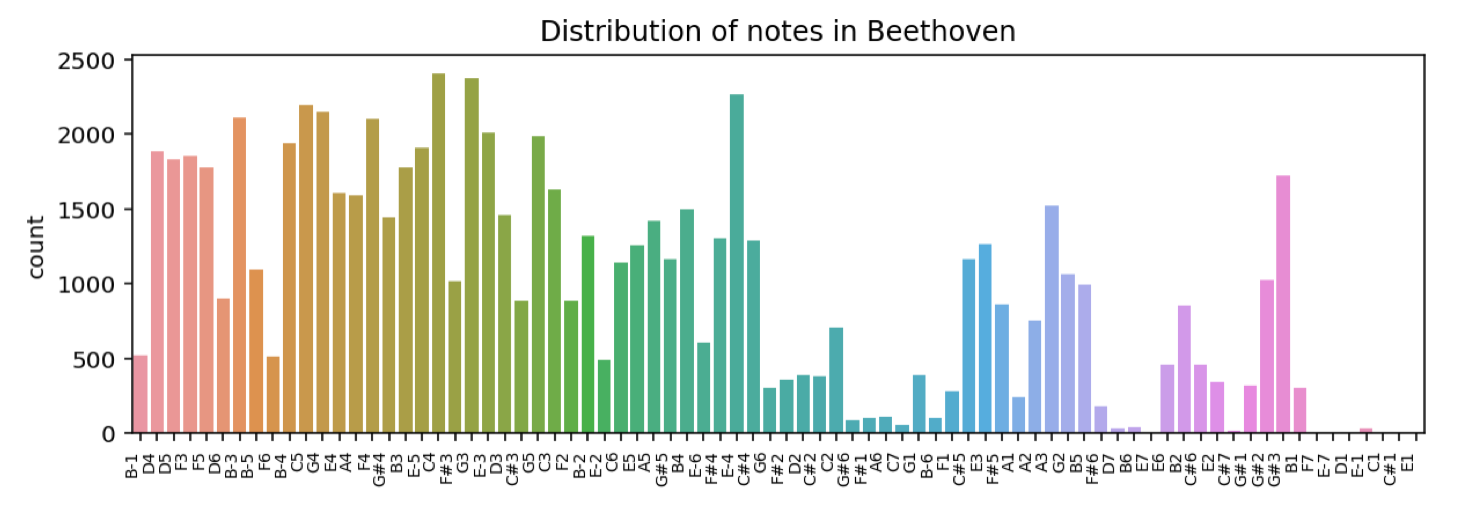
\includegraphics[width = 0.4\textwidth]{note-distribution}

We then featurized the notes/chords as sequences of multi-hot vectors, where we first mapped all unique pitches in song to an index, then transformed individual notes to one-hot vector, and chords to multi-hot vectors (based on pitches).

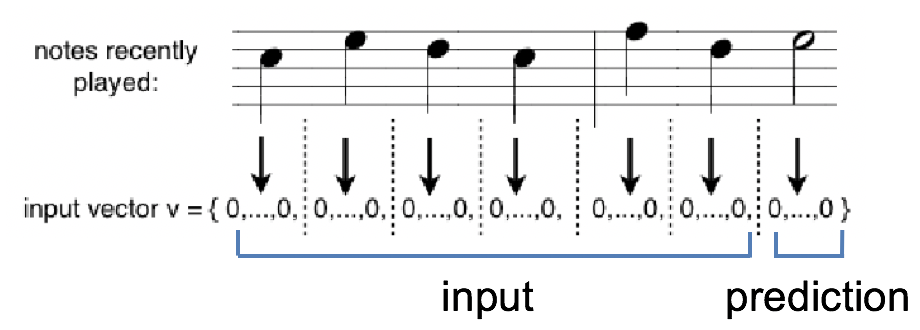
\includegraphics[width = 0.4\textwidth]{one-hot-encoding}

We used a sliding window approach to capture the temporal structure in the data. Our input at each time-step is the vector concatenation of the past 10 notes, and our label is the next note. With our 26 songs, this yields a total of 74,593 training examples, which we split into an 85/15 train/dev split.


%------------------------------------------------

\section{Methods}

\subsection{Baseline: Logistic Regression}

We begin with a simple logistic regression classifier trained to output the succesor note to a sequence of notes, encoded in one-hot vector form. Our baseline treats the problem as a multiclass classification problem: there are 78 possible successor notes in our database, and our model emits the most probable successor to a given sequence.

As a brief exploration of the logistic regression model's predictive power, we evaluate its predictive accuracy on our development set. The logistic regression model obtains 28.5\% accuracy in predicting the a sequence's successive note on the Beethoven dataset, and an accuracy of 29.9\% for the Mozart dataset.

Then, to compose a score with our logistic regression model, we feed the model a seed string of notes and repeatedly ask our model to predict a subsequent note. With the subsequent note, we have a new a string of notes which can serve as our model's next generation seed.

\subsection{LSTM}

Our next model a long short-term memory (LSTM) model, which is a refinement on the more general class of recurrent neural network (RNN) models. Recurrent neural networks are designed to capture and remember structure across time. In particular, the input to the model at each timestep is not only the new note, but the hidden state at the previous step of the model. A simplified depiction of an RNN is included below.

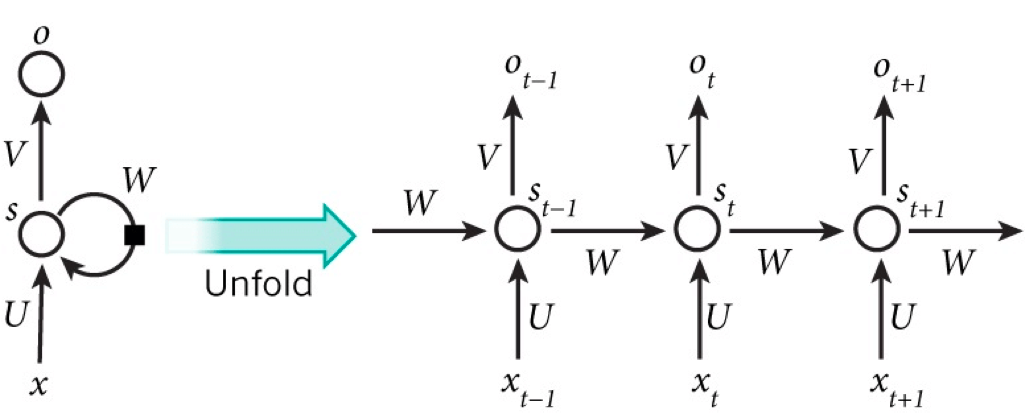
\includegraphics[width = 0.4\textwidth]{rnn-diagram}

LSTMs are a special class of RNNs augmented to better remember long-term dependencies. Within each hidden node, there is an additional cell state and a series of gates which control how much information is updated or forgotten in the cell state. These gates are depicted in the diagram below.

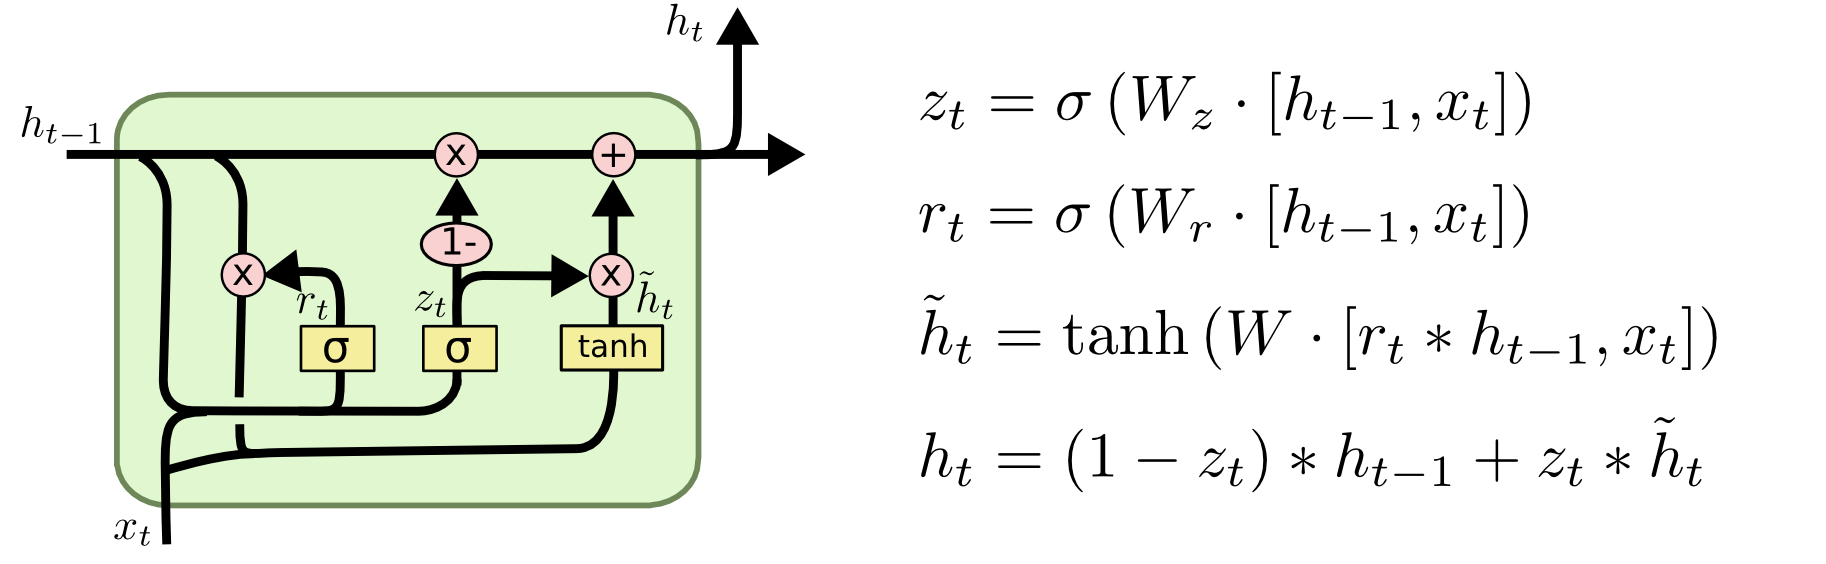
\includegraphics[width = 0.4\textwidth]{colah-lstm-diagram}

*add note on Attention*

%------------------------------------------------

\section{Next Steps}

\subsection{Incorporating Chords and Rhythm}
First and foremost, we intend to extend our models to handle and predict more complicated musical structures, such as chords and rhythms. Right now, our current model only deals with one-hot encoding of single notes. We can handle chords by reframing our problem as a multilabel problem with inputs vectors marked as 1 for every note present, which we are already in the middle of transitioning to.

Similarly, because we are reducing all our training data into sequences of notes, we are currently throwing away all rhythmic information in the data. At generation time, we end up generating one note (or chord) at a time, each with the same length, which does not mimic any rhythm patterns in real music. We have two proposed solutions.

First, at each step, we could have the neural network simultaneously predict the next note and the duration of the next note, and train on both losses simultaneously (tuning the weight of the latter loss to an optimal performance). Another idea would be to discretize the space of note lengths, and at each smallest unit, predict either the next note, or predict a "hold" beat or "rest" beat. If we predict "hold," we would continue with the previous note, and if we predict "rest", there would be no output for that beat. While this idea would require more data preprocessing and significantly simplifying some input songs and rhythmic patterns, it may be much easier to learn, as we only add 2 more classes to the label space instead of a whole separate target to learn and optimize for.

\subsection{Improving the Model}

Firstly, we intend to develop more powerful models to handle the complext structure in musical data. Using the sequence extraction methods described above, we plan to next feed these one-hot encoded sequences into recurrent neural network architectures. We will likely begin with a vanilla Recurrent Neural Nework (RNN), then move to tuning a Long Short-Term Memory network (LSTM), and possibly try generative models such as Variational Autoencoders as well. Improving the performance of these networks will likely require a good deal of hyperparameter tuning and a more diverse training corpus.

Next, we aim to incorporate the music vector embeddings mentioned earlier, developed in previous work on audio processing and composition. We can then feed these embeddings into our models in place of the existing one-hot encodings, which should enhance our models with richer and more accessible information.

Third, we hope to expand our musical range beyond our existing work on the 26-work Beethoven corpus. We may augment our dataset with more classical works, or consider finding a larger corpus in the genres of Jazz or electronica.

Finally, we hope to evaluate our ultimate composition using human evaluators. Previous papers in music generation have used a small number of human evaluators to compare the performance of new models with previous models. This can be measured either by evaluators' personal preference, or how "human" they rate the music to be. We plan to recruit several human testers to compare the acoustic quality of our baseline, neural network model, and human standard.


%------------------------------------------------

\section{Contributions}

Eric handled data preprocessing to extract note sequences from MIDI files and set up the logistic regression baseline. Joyce and Sam have run an LSTM baseline to compose using our Mozart dataset, and are currently testing other instrumental and synthesized datasets.


%----------------------------------------------------------------------------------------
%   REFERENCE LIST
%----------------------------------------------------------------------------------------

%Sets the bibliography style to UNSRT and imports the
%bibliography file "samples.bib".
\bibliographystyle{unsrt}
\bibliography{ref}

%----------------------------------------------------------------------------------------

\end{document}
